\ifdefined\included
\else
\setcounter{chapter}{4} %% Numéro du chapitre précédent ;)
\dominitoc
\faketableofcontents
\fi

\chapter{Interactive Simulator}
\chaptermark{Interactive Simulator}
\label{chap:5}
\minitoc

\section{Introduction}

In order to validate the approach presented in the previous chapter (\ref{chap:4}), we would like to be able to perform collaboratively a task with a simulated robot executing the produced policy. This allowed us to conduct a user study validating the approach which is described in the next chapter (chap.~\ref{chap:6}).

This chapter is a technical description of the interactive simulator I developed. As depicted in fig.~\ref{fig:simu_architecture}, it consists of several components which will be detailed throughout this chapter. 

\begin{figure}[h]
    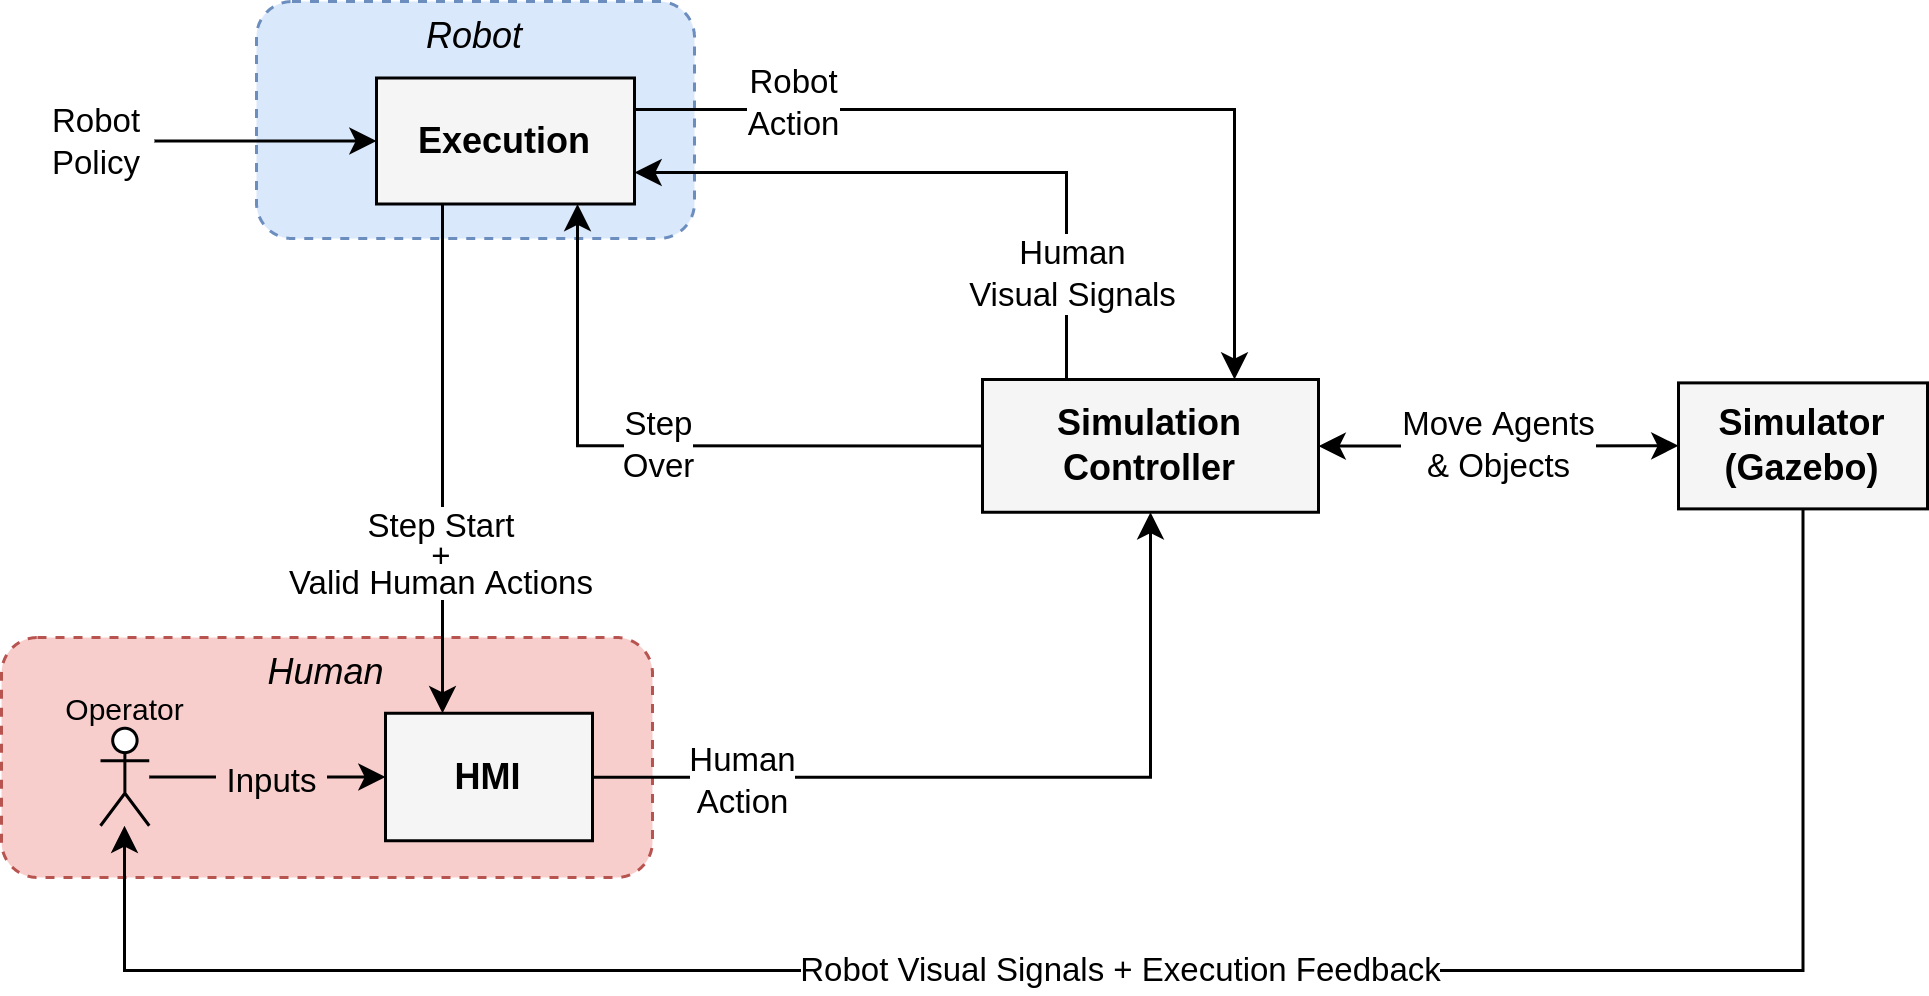
\includegraphics[width=\textwidth]{Chapter6/simu_architecture.png}
    \caption{Overview of the Interactive Simulator's Architecture}
    \label{fig:simu_architecture}
\end{figure}

It consists of an execution and supervision module directly inspired by the model of execution which takes as input a robot policy produced by the concurrent and compliant approach. A simul     


\section{Simulated scene}

This interactive simulator is based on the Gazebo Simulator. It is an open-source 3D simulator able to simulate articulated robots in a dynamic and complex environment.
This section describes all aspects directly linked to this existing 3D simulator our framework has been developed upon.

The static scene consists of a large room, with a ground and 4 walls, and a table placed in the center with two marks on its right side. The marks represent the locations where the cubes must be stacked. The agents are represented as follows. First, the human is represented only with a floating hand as the camera simulates a first-person point-of-view. Then we used a Tiago robot from PAL Robotics because it has an arm to manipulate its environment, a head to send gaze information and signals and because many related resources are available for it (3D models, controllers, tutorials). The human and the robot are facing each other, each from one opposite side of the table. Finally, colored cubes were disposed of on the table in three distinct zones. Cubes are either close to the edge of one of the agents, or they are in the middle of the table. This disposition influences the reachability of the agents as one agent can only reach cubes from their side (just in front of them) or the middle, but never from the other agent's side. This scene corresponds to one specific collaborative task, but another setup could be easily implemented. 

The Gazebo simulator can be integrated with the Robot Operating System (ROS) which is a set of software libraries and tools that help to build robot applications. The main pros of ROS are its ability to run several sub-programs in parallel and make them communicate with each other. Hence, the other components of the interactive simulator have been developed with ROS.

The overall scene is depicted in the figure~\ref{fig:simu_view}. The stacking goal is displayed in the top left corner and a text prompt is shown in the top right corner for the robot to communicate with the human.

\begin{figure}[h]
    \centering
    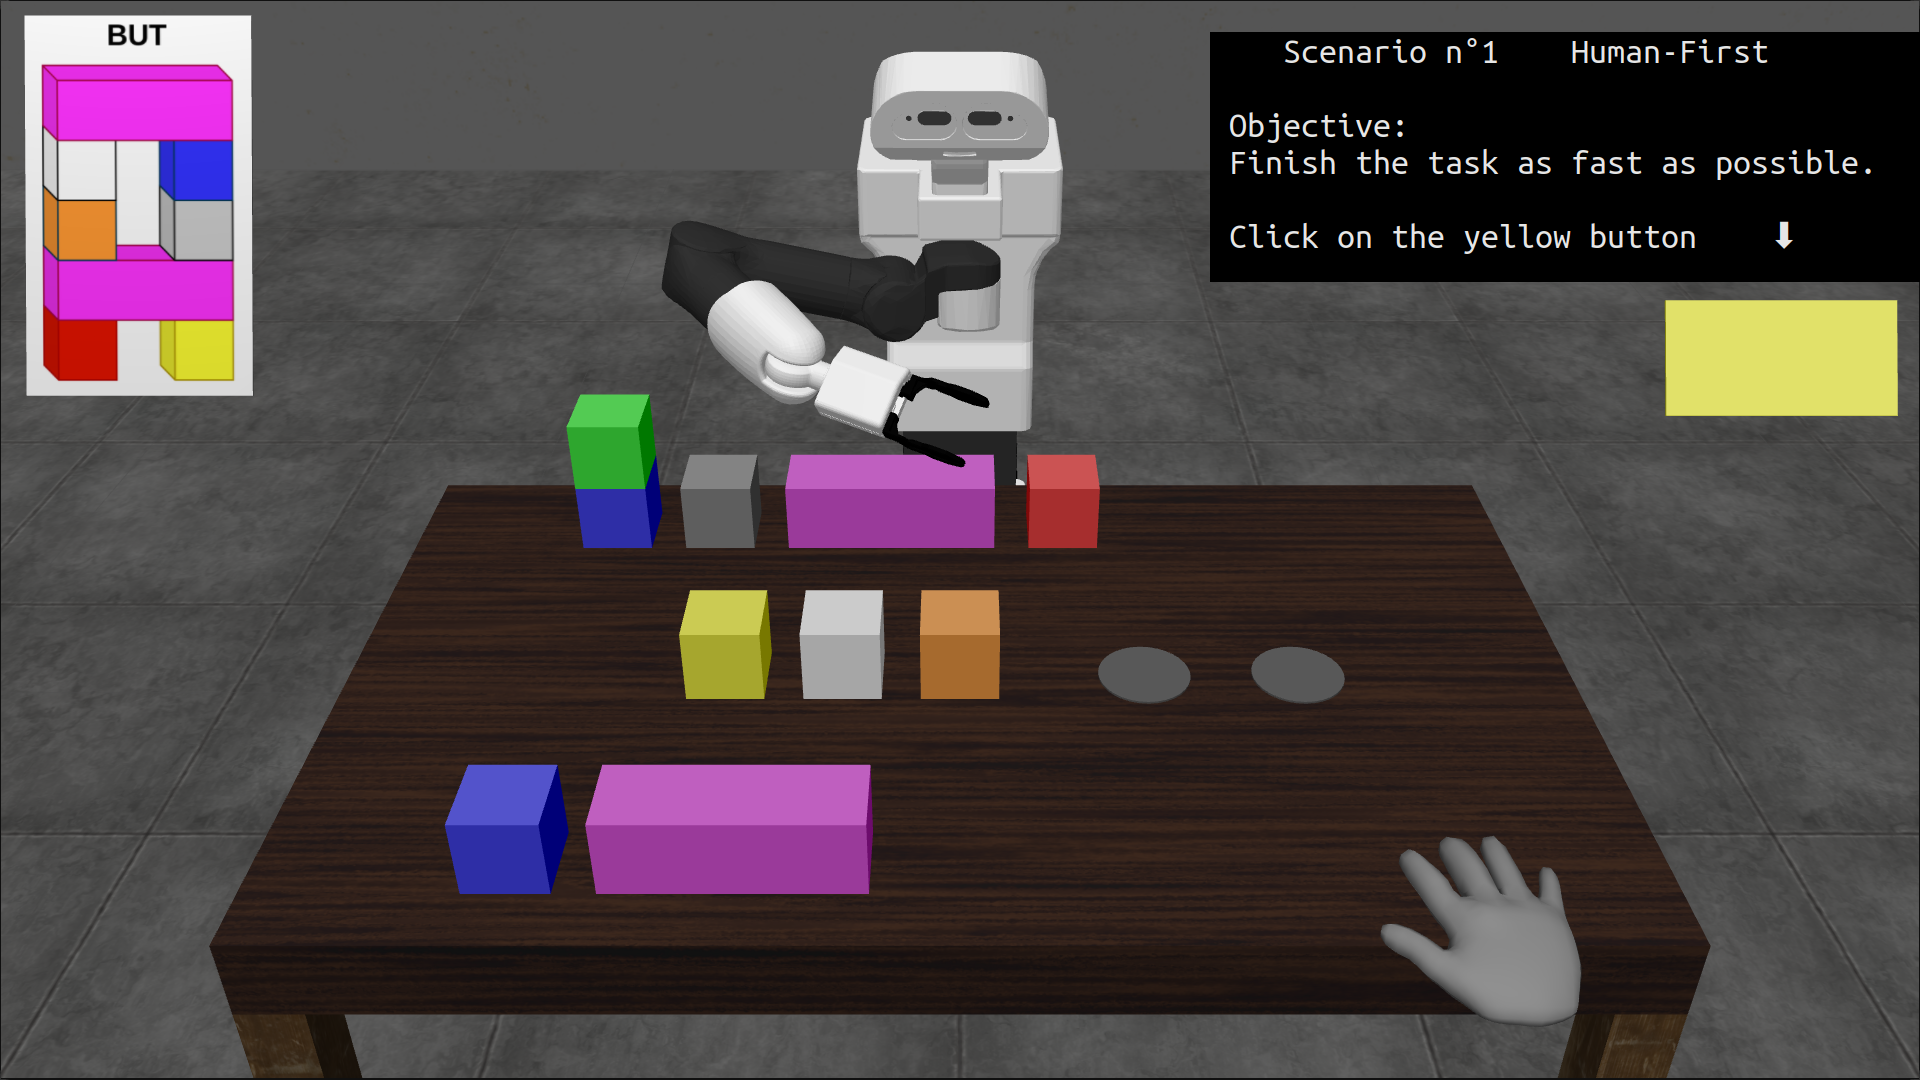
\includegraphics[width=\textwidth]{Chapter6/simu_screenshot.png}
    \caption{Participant view of the interactive simulator. Text prompt. Goal pattern. robot. table. cubes. stacking area. human hand.}
    \label{fig:simu_view}
\end{figure}

\section{Simulation controllers}

To control the simulated agents and the simulation, 4 distinct controllers have been developed and handle dedicated jobs. 

\subsection{Robot arm motion controller}

First, there is one controller to move the robot arm. This controller is called with either a 3D position to reach (pose target) or a predefined configuration (named target). In both cases, when called, this controller uses the MoveIt framework. MoveIt creates links between several libraries in order to have access to a unified interface for Motion Planning algorithms, Inverse Kinematics, Control, or Collision Checking. This way, our controller can ``simply'' request MoveIt to find a trajectory to a given position and then make the robot follow this trajectory while taking into account the geometry of the robot arm.

In fact, this controller is slightly more sophisticated. Indeed, in our collaborative context, we prefer the robot to be reactive rather than to have optimal motions. This is why, through the MoveIt interface, we use two different motion planners. The first one is $RRT^*$ which is an optimal planner that stops only when the optimal motion plan has been found. This is desirable to have the robot exhibit consistent and efficient motions. However, this process sometimes takes too much time (4-5s), which breaks the rhythm of the interaction. As a consequence, a short timeout (0.6s) has been set for this optimal motion planner. If the optimal plan isn't found within the defined timeout, we use the second motion planner. 
The second planner is $SBL$ which isn't an optimal planner. That is, the planner stops when a solution is found, but there is no guarantee of optionality. The major pro of this planner is its speed.
Overall, for every robot arm motion, we first try to find an optimal motion within a short amount of time. If the optimal motion isn't found, we quickly find a suboptimal solution to prevent the robot from being passive for too long.

Additionally, to reduce motion planning time, a few simplifications have been done. 
First, collisions are only considered with the table and the robot's body. Hence, the robot arm sometimes go through the other cubes.
Also, the pick and place orientation are ignored, for instance, when picking a cube the robot gripper just reaches the cube's center from any angle and then the cube is attached to the gripper. When placing a cube, the robot moves the cube to the target position and when dropping it, the cube is detached and both its orientation and position are overwritten to match the actual target location. This way, the robot always performs perfect place action, improving both the reactivity of the robot and its robustness, but the robot's motions are less realistic.

\subsection{Robot head motions}

To exhibit a more intuitive and collaborative behavior, the robot head is controlled to look at various elements during the interaction. 
Indeed, when waiting for the human the robot looks at the camera, and as soon as the human hand moves to either perform an action or indicate its passivity, the robot starts following the hand to show it is observing the human motions to understand their intentions.
Then, the robot looks at a cube to indicate its intention to pick it since this is faster than the arm motion. 
Also, the robot looks at the target position when placing a cube to indicate its intention to place the cube there.

To perform those head motions a dedicated controller has been developed based on an existing controller provided in the Tiago robot modules. The existing controller could only change the robot's gaze through a visual and clickable window allowing an operator to manually click on the scene to change the robot's gaze. This controller has been modified to allow additional features such as directly requesting to look at 3D point or an object. But also, we can now ask to follow an object. That's how we are able to exhibit the head behavior described just above.  

\subsection{Human hand motions}

Moving the human hand requires a dedicated controller but is much simpler than the robot arm motion one. Here, the hand must either move to a position or perform a PASS signal. The PASS signal is a hand gesture indicating to the robot that the human desires to be passive for the current step. This motion is performed by simply rotating the hand back and forth at a constant speed. The PASS motion has a duration of 0.7s. 
On the other hand, to move the hand to a target position we do not use a real motion planner. We simply compute a straight line between the current hand pose and the target pose, and update the hand position at $50Hz$ to move at a constant speed set to $0.25 m/s$. The planning time is thus negligible compared to the robot motion planning times.

\subsection{Simulation controller}

\subsubsection{Action decomposition}

Last but not least, I developed a fourth controller whose main job is to translate the actions from the plan produced by our task planner to low-level motions that can be executed by the controllers listed above. Hence, some parts of this controller are domain-specific, but a major part is generic for manipulation tasks. This controller received high-level agent actions to execute such as ``Robot pick(b1)'' for the robot picking the cube b1. The first step is to decompose this action into low-level generic actions which are themselves made of low-level motions. This controller also keeps track of a few low-level facts to check low-level preconditions, such as, what are each agent holding or which object is still on the table. Hence, when an agent tries to pick a cube while already holding a cube the controller throws an error.

Let's first comment the low-level generic actions available. This controller is given a list of the object names (cubes) and the names of some predefined locations in the scene (placing locations in the stack). Note also that many of the following actions can be performed either by the human or the robot, this is defined by a parameter given when calling the action. The following low-level actions are available:

\begin{itemize}
    \item \textbf{move\_pose\_target:}          moves either the hand/robot arm to a given position.
    \item \textbf{move\_location\_target:}      moves either the hand/robot arm to the position of a given location.
    \item \textbf{move\_obj\_target:}           moves the hand/robot arm to the position of a given object.
    \item \textbf{move\_home:}                  puts the agent in its ``home'' (default) configuration. 
    \item \textbf{move\_named\_target:}         moves the robot arm to the given configuration.
    \item \textbf{grab\_obj:}                   attaches the given object to the hand/robot gripper. 
    \item \textbf{drop\_obj:}                   detaches the given object to the hand/robot gripper.
    \item \textbf{set\_obj\_rpy:}               sets the orientation of a given object.
    \item \textbf{set\_obj\_pose:}              sets the position of a given object.
    \item \textbf{delta\_move\_obj:}            sets the position of a given relative to its current position.
    \item \textbf{human\_hand\_gesture:}        makes a hand gesture to indicate passivity.
    \item \textbf{robot\_head\_look\_pose:}     makes the robot look at a given position.
    \item \textbf{robot\_head\_look\_human:}    makes the robot look at the human (camera).
    \item \textbf{robot\_head\_follow\_obj:}    makes the robot follow a given object.
    \item \textbf{robot\_head\_follow\_hand:}   makes the robot follow the human hand.
\end{itemize}

Then the high-level actions, from the plan produced, are the following with their respective simplified low-level decomposition:

\begin{itemize}
    \item \textbf{PickCube:}            Starts by retrieving the cube's current position by sending a request to the Gazebo simulator. If it is the robot, call robot\_head\_look\_obj to look at the cube. Then, call move\_pose\_target with the retrieved cube position. Once over, grab the cube with grab\_obj. After, move\_home is called to retract the robot arm or bring the hand to its initial position. Finally, if it is the robot, it looks to the human with robot\_head\_look\_human.
    
    \item \textbf{PlaceCube:}           Starts by retrieving the position of the target location to stack the cube. If it is the robot, call robot\_head\_look\_pose with this position. Then, we move either the arm or the hand to that position with move\_pose\_target before dropping the cube in the stack with drop\_obj and adjusting its position. After, we go back to the home configuration with move\_home. And for the robot, we look at the human with robot\_head\_look\_human. 
    
    \item \textbf{BePassive:}           The human waves their hand to explicitly be passive, thus, human\_hand\_gesture is called. The robot doesn't move and only display some texts saying the robot wants to be passive. The text prompt mechanism will be described later.
    
    \item \textbf{DropCubeTable:}       When an agent cannot stack a cube they are holding, they can place it back on the table. First, the drop position is defined. It corresponds to the initial position of the cube being held, except for the green one which is initially on top of another cube and has a dedicated drop position. The robot looks at the drop position with robot\_head\_follow\_pose. The hand or the robot arm is moved to the position with move\_pose\_target. The cube is dropped with drop\_obj and its position is adjusted. Then, the agent is put in its home configuration with move\_home, and the robot looks at the human with robot\_head\_look\_human.  
\end{itemize}

\subsubsection{Manage steps}

One last thing, the simulator controller is in charge of indicating when a step is over. Basically, since we do not consider steps where both agents are passive, a step begins when an agent starts an action. And it is over when both agent actions are done. These rules cover many situations such as if the human initially wants to be passive and wave their hand, as a result, the robot starts performing an action which starts the step. Currently, the step would be over as soon as the robot action is over since the human is passive. However, if the human decides anyway to start performing an action concurrently then the step will be over when both the robot and human actions are over. This may imply that if the human starts acting right before the end of the robot action then the robot will just wait for the end of the human action, and thus, the end of the step before the next step begins.  

\subsubsection{Send visual signals}

The model of execution synchronizes the agents based on explicit visual signals such as the start of a step, the start of an action, the end of an action or hand gesture (PASS). Those signals are modeled explicitly inside the system and managed by the simulator controller.

Indeed, when starting an action, the associated visual signal is sent only when the agent starts to move. Hence, we track the arm and hand motions to know when the action is visible to the other agent. Then, when an action is over, the associated visual signal is sent directly. It is worth mentioning that the human will naturally have a reaction time when seeing the robot visual signals (start/end of action, step start). However, so far, the robot doesn't have any reaction time to such symbolic visual signals. Thus, to simulate the delay introduced by a real perception module (here perfectly simulated) the human visual signals are delayed to the robot by reaction time set to 0.3s. This is still quite fast but at least the robot doesn't interpret instantly the human motions.  

\section{Robot execute and supervision}

\textbf{TODO: to develop}

model of execution, progress in the solution graph of the robot policy, sound for synchronization step start

takes as input the solution graph produced by chap.~\ref{chap:4} appraoch. Then, it is basically an implementation of the model of execution, sending and synchronizing on the visual signals produced and sent my the simulator. Hence, we have a durative execution of the plan with an effective effect in the simulated environment.

ID process, best robot concurrent action, TO 

Note that during the planning process described in the previous chapter, the model of execution has been abstracted and taken into account to explore relevant courses of actions by anticipating possible executions. Here, the model of execution is rather implemented, matching the abstraction made, to be able to execute the produced robot policy and supervise its execution by synchronizing with the human.

\section{Human Machine Interface (HMI)}

\textbf{TODO: to develop}

text prompt, clickable zones, signals

Human operator or participant can interact with the simulation by performing any feasible action during the process. The model of execution is still followed, thus, every step starts by the robot sound and a dedicated process receives internally the list of the feasible human actions for the current step. This list is sent by the robot execution scheme which is reading the solution graph. Yet, the feasible actions aren't shown nor known by the participants.
Each possible human action is associated to a zone (rectangle) on the screen. When the human mouse click in a zone associated to a currently feasible action, then the process request the simulation controller to perform the corresponding human action.  delayed visual signal for robot.


% ***********



% First, it is using Gazebo to simulate the scene (table, cubes, agents). 
% The robot is a Tiago robot from PAL Robotics. We used a MoveIt controller to plan and execute arm motions. We used a publicly available component to control the gaze of the robot. The head behavior is ad hoc and designed by us.
% The human agent is simulated only with its hand which is moved with a handmade dedicated controller. 
% For simplicity reasons physics of objects isn't simulated, thus, each agent interact with the scene by statically attaching/detaching object respectively to the robot's gripper or the human hand.
% A higher level component called the simulator controller is in charge of translating primitive actions to low level commands and calling the previously presented controllers to make the agent perform actions. Since it manages agent's action, it is also in charge of sending simulated visual signals and indicating when a step is over. Indeed, the agents synchronize themselves using simulated visual signals, and not internal signals. That is, when the human starts performing an action, a brief motion planning phase occur before effectively moving the hand, the motion visual signal is sent to the robot only at this moment. Moreover, to simulate some real perception aspect, a voluntary reaction time is introduced in the robot. Thus, the visual signal can be treated only after this reaction time is passed. A step starts when one agent starts acting (the human or the robot) and it is over when both agents are inactive. Hence, once one agent started to act the other is free to perform an action concurrently and the step will be over only when both are done. If the other agent doesn't act it will be considered as passive/inactive and the step will be over as soon as the first agent finishes.

% Then we can find the respective agents' components. The robot component is an implemented version of the model of execution. Its purpose is to supervise the policy execution of the robot while running the automaton described in the model of execution. In practice, the robot starts by indicating when the step started with a sound signal. Then, it waits to receive the visual human signals for a defined amount of time. Without any visual signal the human is considered as passive. The human can either start acting (how will be described just after), which will eventually send a visual signal to the robot, or the human can make an explicit hand gesture to indicate to the robot that they will be passive (this doesn't force the human to be passive for the whole step). Note that even if the robot received the human visual signal of the human starting to act, the actual action being performed isn't yet identified, it only means that the human started to act. The robot must perform a dedicated identification process (ID Phase/Process) to identify the human action. We assume that the hand gesture that the human can make is always successfully identified instantly (without ID Process). Once either the signal received or the time-out reached, if the best robot action doesn't depend on the human decision then the robot can directly start executing this action. The robot action choice is sent to the simulator controller that will start executing the action. If the best robot action depends on the human decision then the human decision must be identified and the ID Process is run. Only after the robot can perform the best action indicated by the policy which is compliant with the identified human action. If the ID Process fails then the robot remains passive, this case is already part of the policy.
% Eventually the robot waits for the step over signal from the simulator controller and run the Assessment Process. The latter identify what happened during the step (which action the human performed, even if ID wasn't necessary) and in which state we are to be ready to execute the next step and progress in the policy and toward the goal. 

% The human action execution consists in the following. First, the gazebo simulator is made as the main Human-Machine Interface (HMI). Through a handmade plugin one can mouse click in the gazebo simulator window. The click position is sent on a ROS Topic and treated in a dedicated node to potentially trigger a human action. For instance, clicking on a cube starts a "picking" action with the corresponding cube as parameter, clicking on the stack area starts a "place" action, clicking on the table while holding a cube starts a "hold" action, and clicking on the hand make an explicit hand gesture to signal the robot the human desire to be passive. After clicking the hand once, the participant can click another time to indicate the robot full passivity until further notice. The robot will consider the human as unavailable or even not present and will not wait for them. 
% For this to be possible we did the following. First, another gazebo plugin has been written to lock the GUI camera as a First Person View and avoid the participant to accidentally move the camera.
% Then, at every step, the robot component sends to the component receiving the coordinates of the click the currently valid human actions that the participant can perform. Thus, the participant cannot try to place a cube without holding it. Eventually, each human action is mapped to a clickable zone on the gazebo window. Hence, when the click coordinates are received, we check if it is inside one of the designed zone and is the action associated to the zone is currently valid. If so, then the action decision is sent to the simulator controller to be executed. 
% For clarification purpose, when clicking on a cube the robot doesn't immediately know that the human is picking a cube. First, it will know that the human started to act only after receiving the visual signal (after the defined reaction time). And the robot must perform an additional perception phase (ID Process) to identify which action the human performed. 

% Additionally, the stacking goal pattern is shown inside the simulator and a small prompt overlay is present to simulate a potential screen with which the robot can communicate its intention to the human during the collaboration. 

% Thanks to all these processes, the participant is able to intuitively perform actions using mouse control and can collaborate with the robot to solve the task.

% An integrated tutorial has been made to familiarize the participant with the mouse control and the relevant concepts used in the collaboration (notion of step, able to be passive). 